\section{Analizator sygnałów analogowych - test zaprojektowanego systemu}
Kolejnym etapem projektowania części do pomiaru sygnałów analogowych było przetestowanie 
zaprojektowanie systemu.

\subsection{Opis stanowiska pomiarowego.}
Pomiary systemu wykonano z użyciem generatora DDS FG-100 DDS FUNCTION GENERATOR.
oraz przenośnego oscyloskopu Fnirsi 1c15 jako układu odniesienia z pomocą którego
zadawano parametry generowanych sygnałów. Stanowisko pomiarowe przedstawiono poniżej.

    \begin{figure}[!ht]
        \centering
        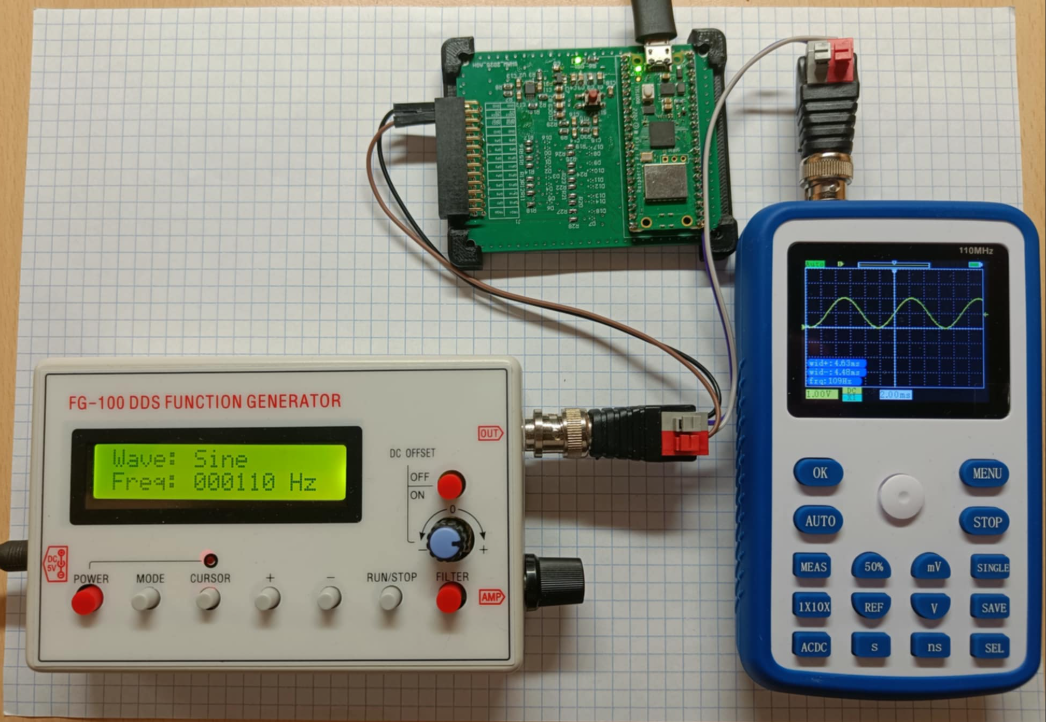
\includegraphics[width = 0.8\textwidth]{stanowisko_pomiarowe.png}
        \caption{Układ stanowiska pomiarowego}
        \label{fig:gui_white}
    \end{figure}

\subsection{Test przetwornika ADS1115}
